\section{Illumination-Guided U-Net Family}

The second model family implemented in this project is an illumination-guided U-Net, introduced as a lightweight mitigation of the local brightness-control failures observed in the baseline. Instead of adding a separate enhancement branch, this variant retains the same general U-Net encoder-decoder design while complementing the low-light RGB image with an estimated illumination map. The selected configuration uses a compact four-level backbone, so the comparison with the final classical U-Net is a family-level comparison under the same protocol, rather than a strict input-only ablation. This idea is related to illumination-guided encoder-decoder enhancement models~\cite{DBLP:journals/corr/abs-2507-13360}, but it is deliberately simplified here in order to test the effect of providing explicit illumination information.

\subsection{Architecture}

The illumination-guided U-Net preserves the general encoder-decoder structure described in the previous section. Therefore, it still uses convolutional blocks, downsampling stages, upsampling stages, skip connections, and a final sigmoid output in the $[0,1]$ range. The output is also unchanged: the model still predicts a three-channel enhanced RGB image. The selected configuration uses the compact four-level channel schedule $(32,64,128,256)$, group normalization, and transposed-convolution upsampling, for a total of $1.93$M trainable parameters. It is therefore smaller than the final classical U-Net, which has $7.76$M trainable parameters.

The difference is at the input level. In the baseline U-Net, each image is represented by three channels, corresponding to red, green, and blue. In the illumination-guided U-Net, a fourth channel is concatenated to these RGB channels. This fourth channel is the estimated illumination map, i.e., a single-channel image that assigns one brightness value to each spatial position. Its purpose is to tell the network which regions are darker, which regions are already relatively bright, and where illumination may be uneven.

No ground-truth illumination annotation is required. The map is computed directly from the low-light input image. During training, this computation is performed after online data augmentation. Therefore, the illumination map is estimated from the same augmented input that is actually passed to the model. This is important because the fourth channel must remain consistent with the RGB image seen by the network. During validation and test evaluation, where no online augmentation is applied, the map is computed from the deterministic preprocessed input.

Two simple illumination estimators are considered. The first one is based on luminance, computed with the same ITU-R BT.709 luma definition used during preprocessing and diagnostic evaluation in Eq.~\ref{eq:luminance}.

The second estimator is based on the maximum RGB response:
\begin{equation}
	L_{\max,i,j}
	=
	\max\left(R_{i,j}, G_{i,j}, B_{i,j}\right).
	\label{eq:max_rgb_res}
\end{equation}
This choice follows the intuition that, at each pixel, the brightest color channel provides a simple estimate of the local amount of light. Similar maximum-channel illumination estimates have been used in low-light enhancement methods based on illumination map estimation~\cite{DBLP:journals/tip/GuoLL17}.

The illumination map can optionally be smoothed before being concatenated to the RGB image. Smoothing is performed with a Gaussian blur, which replaces each value with a weighted average of nearby values, giving more importance to pixels close to the center and less importance to farther pixels. In this work, Gaussian smoothing is included because illumination is expected to vary more slowly than texture, noise, or object edges. Without smoothing, the fourth channel may contain high-frequency details that are not really illumination, such as fine texture or sensor noise. With smoothing, the map becomes more focused on the broad brightness distribution of the scene.

The smoothing option is controlled by the size of the Gaussian kernel. A value equal to zero disables smoothing, while a positive odd value enables it. Odd kernel sizes are used because they define a symmetric window with a well-defined central pixel. This is useful for Gaussian filtering, since the weights are distributed around the center of the window. In the grid search, the smoothed version uses a $9 \times 9$ Gaussian kernel with standard deviation $\sigma = 1.5$. The kernel size defines the spatial support of the filter, while $\sigma$ controls how quickly the weights decrease as the distance from the center increases: smaller values make the smoothing more local, whereas larger values produce a stronger blur. The smoothing option is configurable because excessive smoothing may remove useful local illumination changes, especially near shadows or light sources.

Once estimated, the illumination map is appended to the RGB image, producing a four-channel input. As a result, only the first convolutional layer must be adapted to receive one additional channel; for a fixed channel schedule, the remaining layers follow the same U-Net construction. Therefore, for any fixed backbone configuration, the illumination-guided variant introduces only a minimal parameter increase, confined to the first convolutional block.

The expected benefit is better local brightness control. In dark regions, the illumination cue may help the network apply a stronger correction. In already bright regions, it may help the network avoid unnecessary amplification. Therefore, the model is expected to reduce residual darkness, limit over-exposure around local light sources, and adapt the enhancement more locally than the baseline U-Net.

\subsection{Training Objective and Grid Search}

The illumination-guided U-Net follows the same experimental protocol used for the baseline family. The training objective is kept unchanged in order to isolate the effect of the illumination cue. Therefore, the model is trained with the same L1-SSIM loss defined in Eq.~\ref{eq:l1_ssim_loss}. The loss still compares the predicted RGB image with the paired normally exposed target. The illumination map is used only as additional input information; it is not supervised by a separate target and does not introduce an additional loss term.

The grid search uses the same screening budget as the baseline U-Net, with 144 configurations. However, the search space is made family-specific: upsampling and weight decay are fixed to the values selected by the baseline U-Net, while the freed budget is used to explore the illumination estimator and the smoothing option. The explored hyperparameter space is:

\begin{itemize}[topsep=5pt]
	\item Channel schedule $\in$ $(16,32,64,128)$, $(32,64,128,256)$, $(32,64,128,256,512)$;
	\item Normalization $\in$ none, batch, instance, group;
	\item Learning rate $\in$ $3{\cdot}10^{-4}$, $5{\cdot}10^{-4}$, $10^{-3}$;
	\item Illumination estimator $\in$ luminance, maximum RGB response;
	\item Illumination smoothing $\in$ disabled, Gaussian blur with $9 \times 9$ kernel and $\sigma = 1.5$.
\end{itemize}

\subsection{Quantitative Analysis}

This subsection reports the quantitative behavior of the selected illumination-guided U-Net family. The final configuration is the one selected by the fixed experimental protocol of this project, and has $1.93$M trainable parameters. Table~\ref{tab:illumination_guided_unet_final_evaluation} reports the final evaluation of the selected illumination-guided U-Net configuration.

\begin{table*}[t]
	\centering
	\caption{Final evaluation of the selected illumination-guided U-Net configuration. The first row reports the held-out in-domain evaluation, the following three rows report independent external evaluation results, and LOL-v1 (overlap) is reported for descriptive transparency only and is excluded from independent cross-dataset conclusions. Values are reported as mean $\pm$ standard deviation across three seeds. Full-reference metrics are not available for ExDark because it is unpaired.}
	\label{tab:illumination_guided_unet_final_evaluation}
	\resizebox{\textwidth}{!}{
		\begin{tabular}{lccccccccccc}
			\toprule
			Dataset & SSIM & PSNR (dB) & MAE & NIQE & BRISQUE & Mean $Y$ & Std $Y$ & Dark (\%) & Clip (\%) & RGBI & Lap. sharp. \\
			\midrule
			LOL-v2 Real & $0.841 \pm 0.013$ & $19.00 \pm 0.96$ & $0.112 \pm 0.012$ & $6.59 \pm 0.20$ & $27.86 \pm 0.41$ & $0.464 \pm 0.017$ & $0.164 \pm 0.003$ & $1.0 \pm 0.3$ & $0.09 \pm 0.02$ & $0.039 \pm 0.002$ & $0.0089 \pm 0.0002$ \\
			\midrule
			LOL-v2 Synthetic & $0.761 \pm 0.015$ & $17.29 \pm 0.39$ & $0.127 \pm 0.007$ & $7.07 \pm 0.17$ & $32.00 \pm 0.86$ & $0.448 \pm 0.013$ & $0.211 \pm 0.006$ & $3.0 \pm 2.7$ & $0.10 \pm 0.01$ & $0.041 \pm 0.007$ & $0.0094 \pm 0.0003$ \\
			MILLs & $0.744 \pm 0.031$ & $16.72 \pm 0.91$ & $0.144 \pm 0.018$ & $6.08 \pm 0.15$ & $24.54 \pm 2.86$ & $0.477 \pm 0.026$ & $0.121 \pm 0.007$ & $0.6 \pm 0.1$ & $0.00 \pm 0.00$ & $0.089 \pm 0.013$ & $0.0060 \pm 0.0006$ \\
			ExDark & -- & -- & -- & $6.94 \pm 0.05$ & $33.85 \pm 0.91$ & $0.417 \pm 0.014$ & $0.195 \pm 0.007$ & $3.4 \pm 2.6$ & $0.13 \pm 0.01$ & $0.078 \pm 0.009$ & $0.0075 \pm 0.0001$ \\
			\midrule
			LOL-v1 (overlap) & $0.882 \pm 0.009$ & $22.15 \pm 0.67$ & $0.076 \pm 0.007$ & $6.75 \pm 0.04$ & $29.52 \pm 0.71$ & $0.476 \pm 0.017$ & $0.181 \pm 0.004$ & $2.5 \pm 0.5$ & $0.05 \pm 0.01$ & $0.055 \pm 0.005$ & $0.0085 \pm 0.0002$ \\
			\bottomrule
		\end{tabular}
	}
\end{table*}

\analysispar{In-domain and cross-dataset evaluation}
Since the training protocol is unchanged, LOL-v2 Real remains the in-domain reference. On this dataset, the illumination-guided U-Net obtains $0.841$ SSIM, $19.00$ dB PSNR, and $0.112$ MAE. These values show that the additional illumination channel does not automatically improve paired reconstruction on the source distribution. The model still learns a valid enhancement mapping, but its in-domain full-reference scores are slightly weaker than the baseline U-Net. This suggests that the explicit illumination cue changes the way the network distributes brightness, but it does not by itself make the RGB reconstruction closer to the paired target.

On LOL-v2 Synthetic, the model obtains $0.761$ SSIM and $0.127$ MAE, confirming that synthetic degradation differs from real low-light acquisition used for training. The drop is stronger on MILLs, with $0.744$ SSIM, $16.72$ dB PSNR, and $0.144$ MAE. This shows that the illumination cue alone cannot recover the paired target when acquisition conditions and illumination distribution differ from LOL-v2 Real.

The diagnostic metrics clarify what the illumination map changes. MILLs has the largest RGB imbalance in the table, $0.089$. ExDark becomes brighter and less dark overall: mean luminance is $0.417$ and the dark-pixel ratio is $3.4\%$. This is consistent with the intended mitigation, because ExDark was one of the cases where the baseline left many regions under-exposed. However, this improvement is not free. ExDark still has high BRISQUE, $33.85$, and a relatively high RGB imbalance, $0.078$. Therefore, the illumination-guided input helps the model expose dark regions more aggressively, but does not guarantee better naturalness, color balance, or target fidelity.

Finally, LOL-v1 is reported only as a non-independent overlap-control result. It is excluded from independent cross-dataset interpretation because its low-light inputs overlap with LOL-v2 Real.

\analysispar{MILLs illumination-level analysis}
MILLs is paired, and its illumination-level metadata makes it possible to analyze how the illumination-guided U-Net behaves as input brightness changes. Table~\ref{tab:illumination_guided_unet_mills_illumination} reports the results grouped by illumination level.

\begin{table*}[t]
	\centering
	\caption{MILLs illumination-level results for the selected illumination-guided U-Net configuration. Values are reported as mean $\pm$ standard deviation across three seeds. MILLs is paired, so full-reference, no-reference, and diagnostic metrics are reported. Bold values mark the best score for each full-reference and no-reference metric.}
	\label{tab:illumination_guided_unet_mills_illumination}
	\resizebox{\textwidth}{!}{
		\begin{tabular}{cccccccccccc}
			\toprule
			Level & SSIM & PSNR (dB) & MAE & NIQE & BRISQUE & Mean $Y$ & Std $Y$ & Dark (\%) & Clip (\%) & RGBI & Lap. sharp. \\
			\midrule
			1 & $0.690 \pm 0.013$ & $16.77 \pm 0.61$ & $\mathbf{0.130 \pm 0.011}$ & $6.00 \pm 0.03$ & $\mathbf{20.97 \pm 2.39}$ & $0.461 \pm 0.019$ & $0.169 \pm 0.005$ & $1.8 \pm 0.3$ & $0.00 \pm 0.00$ & $0.092 \pm 0.011$ & $0.0083 \pm 0.0008$ \\
			2 & $0.729 \pm 0.028$ & $16.12 \pm 0.87$ & $0.153 \pm 0.017$ & $\mathbf{5.98 \pm 0.18}$ & $24.27 \pm 2.81$ & $0.492 \pm 0.023$ & $0.130 \pm 0.005$ & $0.9 \pm 0.4$ & $0.00 \pm 0.00$ & $0.092 \pm 0.013$ & $0.0064 \pm 0.0006$ \\
			3 & $0.743 \pm 0.032$ & $16.43 \pm 0.90$ & $0.150 \pm 0.017$ & $6.09 \pm 0.17$ & $24.49 \pm 3.08$ & $0.486 \pm 0.025$ & $0.120 \pm 0.006$ & $0.8 \pm 0.2$ & $0.00 \pm 0.00$ & $0.090 \pm 0.013$ & $0.0059 \pm 0.0006$ \\
			4 & $0.748 \pm 0.033$ & $16.56 \pm 0.92$ & $0.148 \pm 0.018$ & $6.08 \pm 0.14$ & $24.92 \pm 3.02$ & $0.482 \pm 0.026$ & $0.116 \pm 0.006$ & $0.6 \pm 0.1$ & $0.00 \pm 0.00$ & $0.090 \pm 0.014$ & $0.0057 \pm 0.0005$ \\
			5 & $0.751 \pm 0.034$ & $16.70 \pm 0.96$ & $0.146 \pm 0.019$ & $6.09 \pm 0.17$ & $24.96 \pm 2.96$ & $0.479 \pm 0.027$ & $0.114 \pm 0.007$ & $0.5 \pm 0.1$ & $0.00 \pm 0.00$ & $0.089 \pm 0.014$ & $0.0056 \pm 0.0005$ \\
			6 & $0.753 \pm 0.034$ & $16.81 \pm 0.97$ & $0.144 \pm 0.019$ & $6.09 \pm 0.18$ & $25.02 \pm 2.95$ & $0.477 \pm 0.027$ & $0.113 \pm 0.007$ & $0.4 \pm 0.1$ & $0.00 \pm 0.00$ & $0.089 \pm 0.014$ & $0.0056 \pm 0.0005$ \\
			7 & $0.755 \pm 0.034$ & $16.87 \pm 0.98$ & $0.143 \pm 0.019$ & $6.10 \pm 0.18$ & $25.13 \pm 2.98$ & $0.475 \pm 0.027$ & $0.112 \pm 0.007$ & $0.4 \pm 0.1$ & $0.00 \pm 0.00$ & $0.088 \pm 0.014$ & $0.0055 \pm 0.0005$ \\
			8 & $0.756 \pm 0.035$ & $16.92 \pm 0.97$ & $0.142 \pm 0.019$ & $6.14 \pm 0.17$ & $25.19 \pm 2.93$ & $0.474 \pm 0.027$ & $0.112 \pm 0.007$ & $0.3 \pm 0.1$ & $0.00 \pm 0.00$ & $0.088 \pm 0.014$ & $0.0055 \pm 0.0005$ \\
			9 & $\mathbf{0.759 \pm 0.035}$ & $\mathbf{17.04 \pm 0.96}$ & $0.140 \pm 0.019$ & $6.14 \pm 0.21$ & $25.20 \pm 2.91$ & $0.474 \pm 0.027$ & $0.111 \pm 0.007$ & $0.3 \pm 0.1$ & $0.00 \pm 0.00$ & $0.088 \pm 0.014$ & $0.0055 \pm 0.0005$ \\
			10 & $0.757 \pm 0.035$ & $17.00 \pm 0.97$ & $0.141 \pm 0.019$ & $6.13 \pm 0.20$ & $25.30 \pm 2.97$ & $0.472 \pm 0.027$ & $0.111 \pm 0.007$ & $0.2 \pm 0.1$ & $0.00 \pm 0.00$ & $0.087 \pm 0.014$ & $0.0054 \pm 0.0005$ \\
			\bottomrule
		\end{tabular}
	}
\end{table*}

The illumination-level results show a clear dependence on the severity of the input illumination. Level 1 is the hardest case in terms of structural similarity, with SSIM equal to $0.690$. From level 2 onward, SSIM progressively increases and reaches its maximum at level 9. PSNR follows the same general tendency and also peaks at level 9. This means that the model is more faithful to the paired target when the input is not extremely under-exposed.

The MAE result requires careful interpretation. Level 1 has the lowest MAE but also the lowest SSIM, showing that average absolute error can be small even when structure and local contrast are poorly recovered. Thus, MAE should not be read alone: an output may match average intensity while remaining blurred or structurally inaccurate.

Diagnostic metrics show that the illumination-guided model brightens MILLs more strongly than the baseline U-Net. Mean luminance is about $0.477$, and the dark-pixel ratio falls from $1.8\%$ at level 1 to $0.2\%$ at level 10, reducing residual darkness. However, RGB imbalance remains high ($0.087$--$0.092$) across levels and full-reference scores do not improve. Thus, more aggressive exposure correction is not sufficiently constrained to preserve color and target structure under dataset shift.

\analysispar{ExDark category-level analysis}
ExDark is further analyzed by object category because it is unpaired and category metadata is available. Table~\ref{tab:illumination_guided_unet_exdark_category} reports the category-level no-reference and diagnostic results.

\begin{table*}[t]
	\centering
	\caption{ExDark category-level results for the selected illumination-guided U-Net configuration. Values are reported as mean $\pm$ standard deviation across three seeds. ExDark is unpaired, so only no-reference and diagnostic metrics are reported. Bold values mark the best score for each no-reference metric.}
	\label{tab:illumination_guided_unet_exdark_category}
	\resizebox{\textwidth}{!}{
		\begin{tabular}{lcccccccc}
			\toprule
			Category & NIQE & BRISQUE & Mean $Y$ & Std $Y$ & Dark (\%) & Clip (\%) & RGBI & Lap. sharp. \\
			\midrule
			Bicycle & $6.51 \pm 0.06$ & $\mathbf{31.41 \pm 1.05}$ & $0.424 \pm 0.016$ & $0.191 \pm 0.007$ & $2.5 \pm 2.1$ & $0.10 \pm 0.01$ & $0.080 \pm 0.008$ & $0.0093 \pm 0.0002$ \\
			Boat & $7.79 \pm 0.20$ & $35.17 \pm 0.82$ & $0.427 \pm 0.014$ & $0.194 \pm 0.007$ & $4.0 \pm 1.7$ & $0.06 \pm 0.00$ & $0.075 \pm 0.007$ & $0.0079 \pm 0.0001$ \\
			Bottle & $6.76 \pm 0.02$ & $34.32 \pm 1.28$ & $0.403 \pm 0.013$ & $0.196 \pm 0.007$ & $4.5 \pm 3.2$ & $0.16 \pm 0.01$ & $0.089 \pm 0.011$ & $0.0068 \pm 0.0002$ \\
			Bus & $6.47 \pm 0.12$ & $34.82 \pm 0.70$ & $0.405 \pm 0.016$ & $0.192 \pm 0.007$ & $3.2 \pm 2.3$ & $0.14 \pm 0.01$ & $0.085 \pm 0.008$ & $0.0087 \pm 0.0001$ \\
			Car & $7.03 \pm 0.09$ & $34.92 \pm 0.87$ & $0.407 \pm 0.015$ & $0.193 \pm 0.007$ & $3.9 \pm 2.8$ & $0.22 \pm 0.02$ & $0.084 \pm 0.010$ & $0.0068 \pm 0.0001$ \\
			Cat & $6.86 \pm 0.08$ & $32.61 \pm 1.09$ & $0.430 \pm 0.012$ & $0.195 \pm 0.006$ & $2.7 \pm 2.3$ & $0.12 \pm 0.01$ & $0.073 \pm 0.009$ & $0.0067 \pm 0.0002$ \\
			Chair & $7.29 \pm 0.07$ & $34.84 \pm 1.06$ & $0.420 \pm 0.014$ & $0.201 \pm 0.007$ & $3.2 \pm 3.0$ & $0.14 \pm 0.01$ & $0.072 \pm 0.009$ & $0.0076 \pm 0.0001$ \\
			Cup & $7.51 \pm 0.04$ & $37.28 \pm 1.28$ & $0.402 \pm 0.011$ & $0.202 \pm 0.008$ & $5.0 \pm 3.5$ & $0.12 \pm 0.01$ & $0.087 \pm 0.011$ & $0.0061 \pm 0.0002$ \\
			Dog & $6.78 \pm 0.11$ & $32.17 \pm 1.38$ & $0.432 \pm 0.013$ & $0.195 \pm 0.006$ & $2.8 \pm 2.4$ & $0.14 \pm 0.01$ & $0.074 \pm 0.008$ & $0.0070 \pm 0.0002$ \\
			Motorbike & $\mathbf{6.27 \pm 0.04}$ & $31.94 \pm 1.04$ & $0.420 \pm 0.016$ & $0.192 \pm 0.007$ & $3.0 \pm 2.1$ & $0.11 \pm 0.01$ & $0.081 \pm 0.009$ & $0.0086 \pm 0.0002$ \\
			People & $7.04 \pm 0.05$ & $32.73 \pm 1.17$ & $0.406 \pm 0.015$ & $0.193 \pm 0.007$ & $3.4 \pm 2.9$ & $0.17 \pm 0.02$ & $0.071 \pm 0.008$ & $0.0076 \pm 0.0000$ \\
			Table & $6.80 \pm 0.06$ & $35.23 \pm 0.94$ & $0.417 \pm 0.013$ & $0.200 \pm 0.006$ & $3.3 \pm 2.6$ & $0.12 \pm 0.02$ & $0.071 \pm 0.008$ & $0.0077 \pm 0.0002$ \\
			\bottomrule
		\end{tabular}
	}
\end{table*}

The category-level results show that the illumination-guided U-Net reduces residual darkness in several ExDark categories, but difficulty remains uneven. According to NIQE, motorbike is the best category, while boat is the worst. According to BRISQUE, bicycle is the best category, while cup is the worst. Since ExDark is unpaired, these scores do not measure reconstruction against a target. Instead, they indicate how natural or perceptually plausible outputs appear to no-reference estimators. The disagreement between NIQE and BRISQUE also shows that no single no-reference measure fully describes output quality.

The diagnostic metrics show that remaining failures are concentrated in specific scene types. Cup and bottle have the highest dark-pixel ratios, $5.0\%$ and $4.5\%$, meaning that small objects and indoor scenes with strong shadows may remain under-exposed even with the illumination cue. Car and people have the highest clipping ratios, suggesting that reflective surfaces, lamps, or bright local sources can still be over-amplified. Bottle has the highest RGB imbalance, $0.089$, followed closely by cup and bus, consistent with a color-cast risk. These category-specific patterns suggest that errors depend not only on object labels, but also on correlated visual factors such as background darkness, local highlights, and scene composition. Therefore, the illumination map helps with darkness, but it does not separate illumination correction from color preservation and local artifact control.

\analysispar{Summary}
Overall, the quantitative analysis shows that the illumination-guided U-Net only partially solves the failure modes observed in the baseline. The explicit illumination cue reduces residual darkness, especially on ExDark and on the darker MILLs levels. However, this improvement does not translate into a general full-reference gain. In-domain performance on LOL-v2 Real is slightly weaker, MILLs reconstruction quality decreases, and RGB imbalance becomes more visible in cross-dataset settings. Therefore, the illumination channel is useful as a local brightness cue, but it is not sufficient to disentangle exposure correction, color preservation, denoising, and detail fidelity.

\subsection{Qualitative Analysis}

Visual inspection is useful to understand why the illumination-guided U-Net improves some diagnostic brightness indicators but does not improve all reconstruction metrics. Figure~\ref{fig:illumination_guided_unet_qualitative} reports one successful enhancement example and a set of representative failure cases.

\begin{figure*}[p]
	\centering
	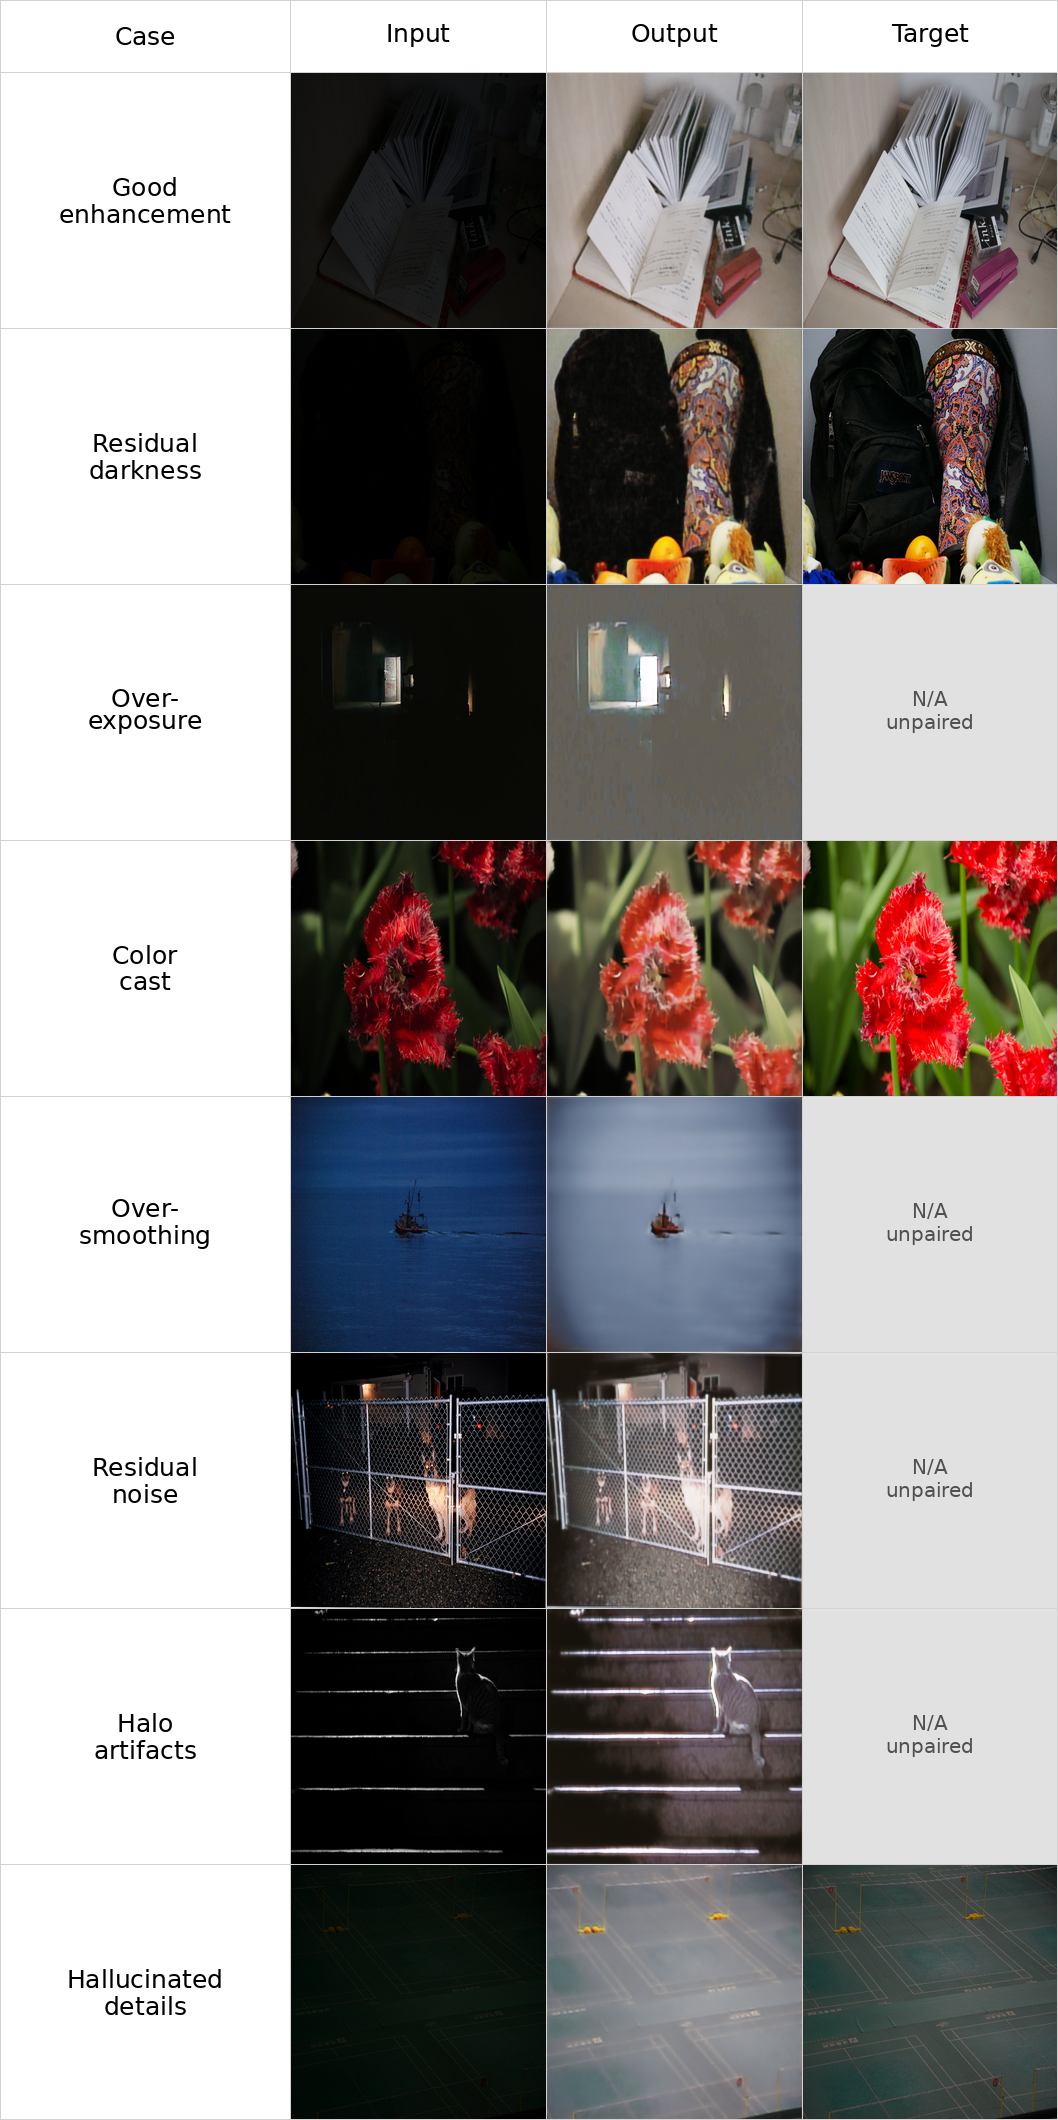
\includegraphics[
	height=\dimexpr\textheight-4\baselineskip\relax,
	keepaspectratio
	]{fig/illumination_guided_unet_qualitative/illumination_guided_unet_qualitative.png}
	\caption{Qualitative examples obtained with the selected illumination-guided U-Net configuration on different datasets used in the project. Each row shows the input, the enhanced output, and the target when available. The rows include one successful enhancement case and representative failure modes: residual darkness, over-exposure, color cast, over-smoothing, residual noise, halo artifacts, and hallucinated details.}
	\label{fig:illumination_guided_unet_qualitative}
\end{figure*}

\analysispar{Hallucinated details}
The hallucinated details example was selected from LOL-v2 Real because the paired target makes the non-faithful content visible. The enhanced output contains a hazy diagonal pattern over the court, while the target is cleaner and more uniform. This is a failure because the model is not only changing brightness, but also introducing visual structure that is not present in the reference. A possible reason is that the input is very dark and contains weak evidence for the true scene. In this situation, the model may produce plausible-looking patterns that reduce the training loss on average but are not faithful to the target.

\analysispar{Color cast}
The color cast example was selected from LOL-v2 Synthetic because the paired target shows the chromatic error clearly. The red flower in the target is vivid and saturated, while the output becomes paler, more orange, and partially shifted toward the green background. This failure is important because it shows that illumination guidance is not the same as color correction. The additional channel mainly describes brightness, not the correct balance between red, green, and blue. A possible reason is that the model is trained on real LOL-v2 images and then tested on a synthetic degradation process with different color statistics, so the learned correction improves exposure but does not preserve the target chromatic distribution.

\analysispar{Over-exposure}
The over-exposure example was selected from ExDark. The input contains a small bright window or light source surrounded by a very dark region. The output makes the scene more visible, but the bright area becomes saturated and the surrounding wall becomes flat and washed out. Since this image comes from ExDark, no paired target is available, but the artifact is visually clear. A possible reason is that the model learns to use the illumination cue to lift dark scenes aggressively, while the loss does not explicitly penalize local clipping. As a result, already bright regions can still be amplified too much.

\analysispar{Over-smoothing}
The over-smoothing example was selected from ExDark. The boat and the sea become brighter, but the output loses fine texture and the whole scene becomes soft. The water surface and the edges around the boat are less detailed than in the input. This effect is especially visible in the sea, where small brightness and texture variations become flatter after enhancement. A possible reason is that the L1-SSIM objective still encourages a safe average reconstruction when details are uncertain. The illumination map helps the model decide where to brighten, but it does not add an explicit constraint that forces fine texture or edges to be preserved.

\analysispar{Residual noise}
The residual noise example was selected from ExDark because the output exposes high-frequency noise and uneven texture after enhancement. The fence and the ground become brighter, but the brightened image also reveals noisy patterns that were less visible in the input. This failure is different from over-smoothing: here the model does not only remove detail, but also amplifies undesirable high-frequency content. A possible reason is that the illumination-guided U-Net is not explicitly noise-aware. When a dark region is brightened, sensor noise is brightened together with real texture, and the current objective does not force the model to separate the two.

\analysispar{Halo artifacts}
The halo artifacts example was selected from ExDark. The cat and the stair edges are surrounded by bright contours after enhancement. This is a typical halo effect: brightness spreads around high-contrast structures and produces an unnatural outline. A possible reason is that the maximum-RGB illumination map can still contain sharp transitions around visible bright edges. If the network uses this cue too directly, it may over-amplify those transitions instead of applying a smooth and edge-aware correction.

\analysispar{Successful enhancement}
The successful-enhancement example is from LOL-v1 (overlap). The input image is strongly under-exposed, but the illumination-guided U-Net recovers the open book, the paper texture, and the objects on the table. The output remains close to the target and does not introduce severe saturation. This example illustrates how the illumination cue behaves on content overlapping with the LOL-v2 Real pool; it is not interpreted as independent transfer evidence.

\analysispar{Residual darkness}
The residual darkness example was selected from LOL-v1 (overlap) because the paired target makes the remaining under-exposure easy to see. The colorful object on the right is enhanced, but the black bag or jacket on the left remains much less visible than in the target. This failure shows that the illumination map does not solve the problem when the input region contains extremely weak signal. A possible reason is that the maximum-RGB illumination estimate can tell the network that a region is dark, but it cannot recover texture that is almost absent from the input. The network can brighten the region, but it still has limited information to reconstruct the missing details faithfully.

\analysispar{Summary}
Qualitative results support the quantitative findings. The illumination-guided U-Net can reduce residual darkness, but may introduce over-exposure, color shifts, smoothing, noise, halos, and hallucinated structures under dataset shift. The LOL-v1 examples are included only as descriptive overlap-control illustrations, whereas independent generalization evidence comes from LOL-v2 Synthetic, MILLs, and ExDark. Illumination guidance is useful, but needs constraints on color, clipping, noise, and edges.

\subsection{Mitigation Strategies}

The results of this family provide an important intermediate test. The mitigation proposed after the baseline U-Net was to provide an explicit local illumination cue. This was useful but insufficient: it reduced residual darkness in several diagnostic results, especially on ExDark, but did not consistently improve full-reference reconstruction and increased the risk of color imbalance and local artifacts. The next mitigation should therefore not only indicate where the image is dark, but also constrain how brightness correction interacts with color, texture, noise, and edges.

A first strategy is to modify the objective in a frequency-aware way. The qualitative failures observed in this family occur at different visual scales. Exposure, color cast, and broad illumination errors are mainly low-frequency phenomena, varying smoothly over large image regions. Texture loss, residual noise, edge sharpness, and halo artifacts are mainly high-frequency phenomena, depending on local details and rapid spatial changes. This motivates a loss that decomposes prediction and target into low- and high-frequency components, penalizing illumination and color errors on the former and detail-related errors on the latter. This direction is inspired by frequency-domain reconstruction losses, which show that spatial losses alone may not sufficiently control frequency content~\cite{DBLP:conf/iccv/JiangDWL21}.

A second strategy is to add exposure consistency. The model should produce compatible outputs when the same input is slightly perturbed with realistic photometric transformations, such as exposure changes, gamma variations, color-temperature shifts, or low-light noise. This is related to low-light enhancement methods using explicit exposure, color, and illumination regularizers rather than only paired pixel-wise supervision~\cite{DBLP:conf/cvpr/GuoLGLHKC20}. It is especially relevant for cross-dataset generalization, as datasets may differ in camera responses, noise levels, and illumination curves. A model stable under mild photometric perturbations is less likely to overfit the acquisition statistics of LOL-v2 Real.

Based on these observations, the next family prioritizes both strategies and introduces Frequency-Aware Exposure-Consistent Low-Light Enhancement (FAC-ECL). Rather than copying a full Retinex-style decomposition, it draws on works separating illumination-related effects from reflectance or degradation-related effects~\cite{DBLP:conf/bmvc/WeiWY018,DBLP:journals/dsp/WeiLL24}. FAC-ECL tests a focused hypothesis: cross-dataset enhancement can improve when training separates low-frequency illumination and color correction from high-frequency detail and artifact control, while encouraging stable predictions under realistic exposure perturbations. The transition thus remains incremental: the baseline U-Net tested a standard encoder-decoder mapping, the illumination-guided U-Net tested whether an explicit brightness cue was sufficient, and FAC-ECL changes supervision to address its unresolved limitations.